% -----------------------------------------  
% Autogenerated LaTeX file from XML DocBook  
% -----------------------------------------  
%%<params>
%% document.language en
%%</params>
\documentclass{report}
\usepackage{ifthen}
\newboolean{DBKIsBook}
\setboolean{DBKIsBook}{true}
\IfFileExists{ifxetex.sty}{%
    \usepackage{ifxetex}%
  }{%
    \newif\ifxetex
    \xetexfalse
  }
  \ifxetex
\usepackage{fontspec}
\usepackage{xltxtra}
\defaultfontfeatures{Mapping=tex-text}
\setmainfont{DejaVu Serif}
\setsansfont{DejaVu Sans}
\setmonofont{DejaVu Sans Mono}
\else
\usepackage[T1]{fontenc}
\usepackage[latin1]{inputenc}
\fi
\usepackage{fancybox}
\usepackage{makeidx}
\usepackage[hyperlink]{dbsimple}
\renewcommand{\DBKreleaseinfo}{}
\setcounter{tocdepth}{5}
\setcounter{secnumdepth}{5}


\renewcommand{\DBKdate}{2016-{}12-{}30}



\title{The Digital Professional, from Startup to Enterprise}
\author{Charles T. Betz}
\hypersetup{%
pdfcreator={DBLaTeX-0.3.7-1},%
pdftitle={The Digital Professional, from Startup to Enterprise},%
pdfauthor={Charles T. Betz}}
% ------------------
% Collaborators
% ------------------
\renewcommand{\DBKindexation}{
\begin{DBKindtable}
\DBKinditem{\writtenby}{Charles T. Betz}
\end{DBKindtable}
}
\makeindex
\makeglossary
\begin{document}
\lstsetup
\frontmatter
\maketitle
\tableofcontents
\listoffigures
\mainmatter

% ------- 
% Chapter 
% ------- 

\chapter{Part I: Founder}
\label{Part-I-intro}\hyperlabel{Part-I-intro}%
  
\label{Sec-I}\hyperlabel{Sec-I} This is the introduction to part I.
 
In this section, we explore the fundamentals of information technology delivery.
 
\textbf{Scenario}
 
You are working in a startup, alone or with one or two partners. You are always in the same room, easily able to carry on a running conversation about your efforts and progress. You have no time or resources to spend on anything except keeping your new system alive and running.
 
\textbf{Chapter 1: IT Value}
 
Chapter 1 introduces you to the fundamental concepts of IT value that serve as a basis for the rest of the course. Why do people want computing (IT) services? What are the general outlines of their structure? How do they come into being? How are they changed over time?
 
All of this is essential to understand for your scenario; you need to understand what computers can do and how they are generally used if you are going to create a product based on them.
 
This chapter also covers the basics of how you'll approach building a product. It's assumed you won't develop an intricate, long-{}range plan but rather will be experimenting with various ideas and looking for fast feedback on their success or failure.
 
\textbf{Chapter 2: IT Infrastructure}
 
In this chapter, you have a general idea for a product and are ready to start building it. But not so fast\ldots{}\hspace{0em}you need to decide some fundamentals first. How will your new product run? What will you use to build it?
 
It's not possible to begin construction until you decide on your tools. This chapter will provide you an overview of computing infrastructure including cloud hosting and various approaches to system configuration.
 
This chapter also presents an overview of source control, as even your infrastructure depends on it in the new world of \textquotedblleft{}infrastructure as code.\textquotedblright{}
 
\textbf{Chapter 3: Application delivery}
 
Finally, you're ready to start building something. While this is not a book on software development or programming languages, it's important to understand some basics and at least see them in action.
 
This is also the \textquotedblleft{}DevOps\textquotedblright{} chapter; it's not just about writing code but about the entire end-{}to-{}end system that gets the code you are writing from your workstation, into collaborative environments, and finally to a state where it can be accessed by end users. From source repository to build manager to package repository to production, we'll cover a basic toolchain that will help you understand modern industrial practices.
 
\textbf{This section's lab approach}
 
While this is not a book about any particular computing language or platform, we need to describe some technical fundamentals. We'll do so in as neutral a manner as possible. However, this book's accompanying labs are based on \href{http://www.ubuntu.com/}{Ubuntu Linux} and \href{https://git-scm.com/}{git}, the distributed version control system created by Linus Torvalds to facilitate Linux development.
 \begin{DBKadmonition}{warning}{Important}
 
Part II, like the other parts, needs to be understood as a unified whole. In reality, digital entrepreneurs struggle with the issues in all three chapters simultaneously.
 \end{DBKadmonition}
 
\section{Chapter 1: IT Value}
\label{Intro-Chap-1}\hyperlabel{Intro-Chap-1}%
  
\subsection{Introduction}
\label{_introduction}\hyperlabel{_introduction}%
  
As noted at the outset, you are a small core of a startup. You are building a product of which IT is a significant part. Your motivations are entrepreneurial; you want to create a successful business. You might be housed within a larger enterprise, but the thought experiment here is that you have substantial autonomy to order your efforts.
You want to do something that has a unique IT component. Regardless of your business, you will need accounting and legal services at a minimum and, very quickly, payroll and HR and so forth. Those things can (and should) be purchased as commodity services if you are a small entrepreneur (I am not aware of any convincing arguments to the contrary, unless you are absolutely on the smallest of shoestring budgets and can work 100-{}hour weeks). Your unique value proposition will be expressed to some degree in unique IT software. While this software may be based on well-{}understood products, the configuration and logic you construct will be all your own. Because of this, you are now a producer (or soon to be) of IT services.
 
Before we can talk about building and managing information technology (IT), we need to understand what it is and why people want it. We'll start this chapter by looking at an IT value experience that may seem very familiar. Then we'll dig further into concepts like the IT stack and the IT service and how they change over time.
 
\subsubsection{Chapter outline}
\label{_chapter_outline}\hyperlabel{_chapter_outline}%
  \begin{itemize}

\item{} An IT value experience
 

\item{} What is information technology?
 

\item{} The IT \emph{service} and the IT \emph{stack}
 

\item{} The IT service
 

\item{} IT changing over time
 

\item{} The digital context
 

\item{} Conclusion
 
\end{itemize}
  
\subsubsection{Learning objectives for this chapter}
\label{_learning_objectives_for_this_chapter}\hyperlabel{_learning_objectives_for_this_chapter}%
  \begin{itemize}

\item{} Explain \textquotedblleft{}IT value\textquotedblright{} in everyday terms
 

\item{} Distinguish between IT service and IT system
 

\item{} Discuss how IT services change over time
 

\item{} Describe various ways of understanding the context in which digital systems are developed and digital value is delivered.
 
\end{itemize}
   
\subsection{What is IT value?}
\label{_what_is_it_value}\hyperlabel{_what_is_it_value}%
  
\label{what-is-IT-value}\hyperlabel{what-is-IT-value}
 
\subsubsection{An IT value scenario}
\label{_an_it_value_scenario}\hyperlabel{_an_it_value_scenario}%
  \begin{figure}[R]

\begin{center}
\imgexists{images/1_01c-women.png}{{\imgevalsize{images/1_01c-women.png}{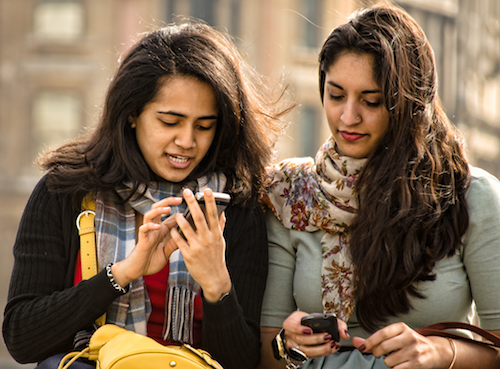
\includegraphics[width=450pt,]{images/1_01c-women.png}}}}{women w/cell phones}
\end{center}
\caption[{Dinner out tonight? }]{Dinner out tonight? \footnotemark{}}
\label{women.png-450-r}\hyperlabel{women.png-450-r}%
\end{figure}
 
Consider the following scenario:
 
A woman is wondering if she can afford to dine out that evening.\footnote{
\emph{Image credit \href{https://www.flickr.com/photos/garryknight/700317885/}{https://www.flickr.com/\-photos/\-garryknight/\-700317885/\-}, downloaded 2016-{}09-{}14, commercial use permitted}
}
 \begin{itemize}

\item{} She uses her mobile device to access her banking information and determines that in fact she does have enough money to do so.
 

\item{} She also uses her mobile device to make a reservation and contact some friends to join her.
 

\item{} Finally, she uses social navigation software to avoid heavy traffic, arriving at the restaurant in time for an enjoyable evening with her friends.
 
\end{itemize}
 
Information technology pervaded this experience. The origins, layers, and complex connections of the distributed systems involved are awe-{}inspiring to consider.
 \begin{DBKadmonition}{warning}{Important}
 
\textbf{Don't worry about the technological terms for now.}  This is an introductory text. You may see terms below that are unfamiliar (model-{}view-{}controller, IP, packet switching). If you are reading this online, you can follow the links, but it's not required. As you progress in your career, you will always be encountering new terminology. Part of what you need to learn is when it's important to dig into it and when you can let it pass for a time. You should be able to understand the gist presented below that these are complex systems based on a wide variety of technologies, some of them old, some new.
 \end{DBKadmonition}
 
The screen on her cell phone represents information accessed and presented via a \href{https://en.wikipedia.org/wiki/Model%E2%80%93view%E2%80%93controller}{model-{}view-{}controller framework}, implemented in the latest version of \href{https://developer.mozilla.org/en-US/docs/Web/JavaScript}{JavaScript}, running on an \href{https://en.wikipedia.org/wiki/Interpreter_(computing)}{interpreter} that would have taxed a \href{https://en.wikipedia.org/wiki/Mainframe_computer}{mainframe} thirty years ago. The communication with her bank's central systems is supported by \href{https://en.wikipedia.org/wiki/LTE_(telecommunication)}{4G LTE} data which in turn relies on the high-{}volume \href{https://en.wikipedia.org/wiki/Internet_Protocol}{IP backbone} networks operated by the \href{http://searchnetworking.techtarget.com/definition/telecom-carrier}{telecommunications carriers}, based on research into \href{https://en.wikipedia.org/wiki/Packet_switching}{packet switching} now approaching fifty years old.
The application operating on the cell phone interacts with core banking systems via sophisticated and highly secure \href{https://en.wikipedia.org/wiki/Middleware}{middleware}, crossing multiple \href{https://en.wikipedia.org/wiki/Computer_network}{network} control points. This middleware talks in turn to the customer demand deposit system that still runs on the mainframe.
 
The mainframe is now running the latest version of \href{https://en.wikipedia.org/wiki/Z/OS}{IBM's z/\-OS} \href{https://en.wikipedia.org/wiki/Operating_system}{operating system} (a direct descendant of \href{https://en.wikipedia.org/wiki/OS/360_and_successors#MVT}{OS/\-360}, one of the most significant operating systems in the \href{https://en.wikipedia.org/wiki/History_of_computing}{history of computing}). The customer demand deposit banking application running on the mainframe is still based on code written in the lowest level \href{https://en.wikipedia.org/wiki/Assembly_language}{assembler}. Some of the comments in this code date back to the 1970s. It has been tuned and optimized over the decades into a system of remarkable speed and efficiency. Although replatforming it is periodically discussed, the cost/benefit ratio for such a project has to date not been favorable.
 
The reservation system looks similar on the mobile device, but the network routes it to a large \href{https://en.wikipedia.org/wiki/Cloud_computing}{cloud} data center hosting the reservation system. The back end application here is very different from the banking system; the \href{https://en.wikipedia.org/wiki/Programming_language}{programming languages} are newer, the \href{https://en.wikipedia.org/wiki/Database}{database} is structured very differently, and the operating system is \href{https://www.linux.com/}{Linux}.
 
Finally, the navigation software looks much like the reservation system, as it too is based on the cloud. However, the system is much more active as it is continually processing inputs from millions of drivers in thousands of cities and updating traffic maps for those drivers in real time so that they can choose the most optimal route to their destinations (e.g., dinner). The capabilities of this system are comparable to an air traffic control system, and yet it is available as a free download for our IT user.
 \begin{figure}[H]

\begin{center}
\imgexists{images/1_01-friends.jpg}{{\imgevalsize{images/1_01-friends.jpg}{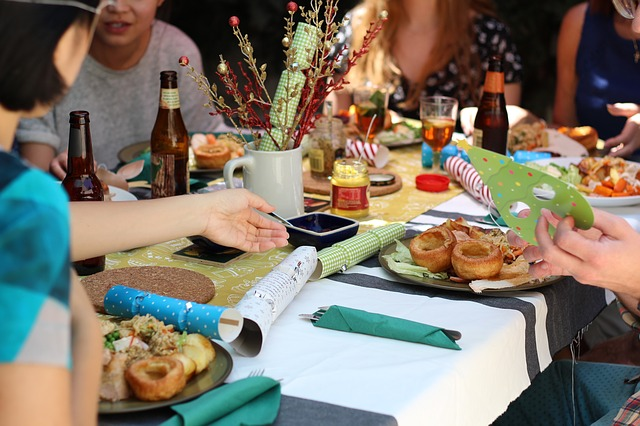
\includegraphics[width=450pt,]{images/1_01-friends.jpg}}}}{party}
\end{center}
\caption[{Digital made this gathering easier }]{Digital made this gathering easier \footnotemark{}}
\end{figure}
 
The resulting value is clear:
 \begin{itemize}

\item{} In an earlier era, our user might have stayed in for fear of bouncing a check, or she might have gone out and dined beyond her means.
 

\item{} The phone line at the restaurant might have been busy, so she might have risked showing up with no reservation.
 

\item{} Before texting and social media, she might not have been able to reach her friends as easily.
 

\item{} Without the traffic application, she might have run into a huge midtown traffic jam and been half an hour late.
 
\end{itemize}
 
Clearly, information technology added value to her life and helped maximize her experience of social enjoyment.
  
\subsubsection{Various forms of IT value}
\label{_various_forms_of_it_value}\hyperlabel{_various_forms_of_it_value}%
  
As we have seen, there are many ways in which digital systems deliver value. Some systems serve as the modern equivalent of file cabinets: massive and secure storage for financial transactions, insurance records, medical records, and the like. Other systems enable the transmission of information around the globe, whether as emails, web pages, voice calls, video on demand, or data to be displayed in a smartphone application (app). Some of these systems support engaged online communities and social interactions with conversations, media sharing, and even massive online gaming ecosystems. Yet other systems enable penetrating analysis and insight by examining the volumes of data contained in the first two kinds of systems for patterns and trends. Sophisticated statistical techniques and cutting-{}edge approaches like neural network-{}based machine learning increase the insights our digital systems are capable of, at a seemingly exponential rate.
 
Digital technology generates value in both direct and indirect ways. People have long consumed (and paid for) communication services, such as telephone services. Broadcast entertainment was a different proposition, however. The consumer (the person with the radio or television) was not the customer (the person paying for the programming to go out over the airwaves). New business models sprung up to support the new media through the sale of advertising air time. In other words, the value proposition was indirect, or at least took multiple parties to achieve: the listener, the broadcaster, and the advertiser. Finally, some of the best known uses of digital technology were and are very indirect\hspace{0.167em}\textemdash{}\hspace{0.167em}the above-{}mentioned banks and insurance agencies using the earliest computers to automate the work of thousands of typists and file clerks.
From these early business models have evolved and blossomed myriads of creative applications of digital technology for the benefit of human beings in their ongoing pursuit of happiness and security. We see the applications mentioned at the outset: online banking, messaging, restaurant reservation, and traffic systems. Beyond that we see the use of digital technology in nearly every aspect of life. (And I say \textquotedblleft{}nearly\textquotedblright{} only because I am a cautious person.)
 
Digital and information technology pervades all of the major industry verticals (e.g., manufacturing, agriculture, finance, retail, healthcare, transportation, services) and common industry functions (e.g., supply chain, human resources, corporate finance, and even IT itself).
 
Digital systems and technologies also are critical components of larger scale industrial, military, and aerospace systems. For better or worse, general purpose computers are increasingly found controlling safety-{}critical infrastructure and serving as an intermediating layer between human actions and machine response. Robotic systems are based on software, and the Internet of Things ultimately will span billions of sensors and controllers in interconnected webs monitoring and adjusting all forms of complex operations across the planet.
    
\end{document}
